\section{The Overall Process of EDG/EDG++}
\label{sec:appendix_algorithm}

In order to clearly describe the proposed EDG/EDG++ framework, we show the overall process in Algorithm~\ref{alg:edg_process}.

\begin{algorithm}[!htb]
   \caption{The overall process of EDG/EDG++ framework.}
   \label{alg:edg_process}
\begin{algorithmic}
   \STATE {\bfseries Input:} Molecular geometries $\mathcal{G}$, ground-truth labels $y$; multi-view ED images $\mathcal{U}$, structural images $\mathcal{S}$.

   \STATE
   \STATE \textbf{Stage I: Pre-training ImageED}
   \STATE Train ED encoder $f_{EDE}$ and decoder $f_{EDD}$ on 2M ED images using:
   \STATE \quad $\mathcal{L}_{ImageED} = \lambda_{VR}\mathcal{L}_{VR} + \lambda_{MR}\mathcal{L}_{MR}$
   \STATE Freeze $f_{EDE}$ after pre-training.

   \STATE
   \STATE \textbf{Stage II: Pre-training ED-aware Teacher and Reliability Estimator}
   \STATE Jointly train ED-aware teacher $f_{\mathcal{S}}$, ED predictor $f_{EDP}$, and reliability estimator $\phi_{eval}$ (EDG++ only):
   \STATE \quad $\mathcal{F}^{\mathcal{S}} = f_{\mathcal{S}}(\mathcal{S})$, $\mathcal{F}^{\mathcal{S}\rightarrow\mathcal{U}} = f_{EDP}(\mathcal{F}^{\mathcal{S}})$
   \STATE \quad $\mathcal{L}_{align} = L1(\mathcal{F}^{\mathcal{S}\rightarrow\mathcal{U}}, \mathcal{F}^{\mathcal{U}})$
   \STATE \quad $\mathcal{L}_{eval} = \mathbb{E}\!\left[\left|\phi_{eval}(\text{detach}(\mathcal{F}^{\mathcal{S}})) - \text{detach}(\|\mathcal{F}^{\mathcal{S}\!\rightarrow\!\mathcal{U}} - \mathcal{F}^{\mathcal{U}}\|_2)\right|\right]$
   \STATE \quad \textit{// detach(): stop gradient; $\phi_{eval}$ receives no gradient from $f_{\mathcal{S}}$ or $f_{EDP}$}
   \STATE \quad $\mathcal{L}_{Stage II} = \mathcal{L}_{align} + \mathcal{L}_{eval}$
   \STATE Freeze $f_{\mathcal{S}}$, $f_{EDP}$, and $\phi_{eval}$ after pre-training.

   \STATE
   \STATE \textbf{Stage III: Downstream Task Training}
   \FOR{each mini-batch $(\mathcal{G}, \mathcal{S}, y)$}
       \STATE Extract geometry features: $\mathcal{F}^{\mathcal{G}} = f_G(\mathcal{G})$
       \STATE Extract structural features: $\mathcal{F}^{\mathcal{S}} = f_{\mathcal{S}}(\mathcal{S})$ (frozen)
       \STATE Compute ED features: $\mathcal{F}^{\mathcal{G}\rightarrow\mathcal{U}} = f_{EDP}(f_M(\mathcal{F}^{\mathcal{G}}))$
       \STATE \quad\quad\quad\quad\quad\quad\quad $\mathcal{F}^{\mathcal{S}\rightarrow\mathcal{U}} = f_{EDP}(\mathcal{F}^{\mathcal{S}})$
       \STATE
       \STATE \textbf{// EDG++: Selective Distillation}
       \STATE Compute confidence: $c_i = -\phi_{eval}(\mathcal{F}^{\mathcal{S},(i)})$
       \STATE Local threshold: $\tau_{local} = \mu_{\mathcal{B}} + \kappa_{batch} \cdot \sigma_{\mathcal{B}}$ \quad ($\mu_{\mathcal{B}}, \sigma_{\mathcal{B}}$: batch mean/std of $\{c_i\}$)
       \STATE Global threshold: $\tau_{global} = \mu_{all} + \kappa_{all} \cdot \sigma_{all}$ \quad (pre-computed over training set)
       \STATE Hybrid threshold: $\tau = \beta \cdot \tau_{local} + (1-\beta) \cdot \tau_{global}$
       \STATE Selection mask: $m_i = \mathbf{1}[c_i \geq \tau]$
       \STATE
       \STATE Compute losses:
       \STATE \quad $\mathcal{L}_{Task} = L1(\hat{y}, y)$
       \IF{$\sum_i m_i > 0$}
           \STATE \quad $\mathcal{L}_{ED} = \frac{\sum_i m_i \cdot SL1(\mathcal{F}^{\mathcal{G}\!\rightarrow\!\mathcal{U}}_i,\, \mathcal{F}^{\mathcal{S}\!\rightarrow\!\mathcal{U}}_i)}{\sum_i m_i}$
       \ELSE
           \STATE \quad $\mathcal{L}_{ED} = 0$ \quad \textit{// skip distillation when no sample is selected}
       \ENDIF
       \STATE Update $f_G$, $f_M$, $f_T$ using $\mathcal{L}_{EDG} = \mathcal{L}_{Task} + \lambda \mathcal{L}_{ED}$
   \ENDFOR

   \STATE
   \STATE \textbf{Inference:} Only use $f_G$ and $f_T$; no ED computation required.

   \RETURN Trained geometry student $f_G$ and task predictor $f_T$
\end{algorithmic}
\end{algorithm}


\section{PyMol Rendering Pipeline}
\label{sec:appendix_pymol}

This section provides the detailed PyMol~\cite{delano2002pymol} commands used for generating multi-view RGB-D electron density images.

\textbf{Structural Loader.} The structural loader uses the command \textit{load \{conformation file\}} in PyMol to load the structural information from the molecular conformation file.

\textbf{ED Loader.} The ED loader uses the commands \textit{load \{ED file\}, ED; load \{ESP file\}, ESP; ramp\_new legend, ESP, [-0.08, 0, 0.08], [red, white, blue]; isosurface surface, ED, 0.05; set surface\_color, legend, surface} in PyMol to load the ED information, which uses a red-white-blue distribution range to describe the electrostatic potential distribution of ED and red, white, and blue represent positive, neutral, and negative regions, respectively.

\textbf{Multi-view Joint Render.} Multi-view joint render uses commands \texttt{set transparency, 0.4; turn \{axis\}, \{angle\}; png \{path\}, width=\{width\}, height=\{height\}} in PyMol to render the ED information and structural information into multi-view RGB-D ED images $\mathcal{U}\in\mathbb{R}^{6\times 4\times 224\times 224}$. Specifically, $\{axis\}$ and $\{angle\}$ represent the rotation angle degrees along axis and we set ($\{axis\}, \{angle\}$) to $(x, 0)$, $(x, 180)$, $(x, 90)$, $(x, -90)$, $(y, 90)$, $(y, -90)$, which means generating images from 6 different views. $\{width\}=224$ and $\{height\}=224$ represent the width and height of the rendered image.

\textbf{Structural Render.} The structural render uses the command template \textit{turn \{axis\}, \{angle\}; png \{path\}} in PyMol to render molecular structures from 2 million conformations into multi-view structural images $\mathcal{S}$. We generate 4 views with $(\{axis\}, \{angle\})$ set to $(x, 0), (x, 180), (y, 180), (z, 180)$.


\section{Markov Assumption and Probability Derivation}
\label{sec:appendix_markov}

We provide the full probability derivation for the ED-aware teacher. Let $s$, $x$, and $h$ denote the molecular conformation, DFT-computed ED data, and ED features, respectively. The acquisition of ED features follows the path $s\xrightarrow{\text{DFT}}x\xrightarrow{\text{ImageED}}h$.

According to the probability chain rule, the joint probability distribution $p(h,x|s)$ can be decomposed into:
\begin{equation}
p(h,x|s)=p(h|x,s)\cdot p(x|s)
\end{equation}

According to the Markov hypothesis~\cite{markov1960theory}, since $h$ is generated from $x$ via ImageED without additional dependence on $s$, we have $p(h|x,s)=p(h|x)$. Marginalizing over $x$:
\begin{equation}
p(h|s)=\int p(h|x)\cdot p(x|s) dx
\end{equation}

Since both stages of the pipeline are deterministic given their inputs---DFT maps $s$ to a unique $x$, and ImageED maps $x$ to a unique $h$---the conditional distributions collapse to point masses: $p(x|s)\approx\delta(x - \text{DFT}(s))$ and $p(h|x)\approx\delta(h - f_{EDE}(x))$. The integral therefore reduces to $p(h|s)\approx\delta(h - f_{EDE}(\text{DFT}(s)))$, which motivates directly learning the composite mapping $s\mapsto h$. The Markov assumption $p(h|x,s)=p(h|x)$ holds exactly when the ImageED encoder is a deterministic function of $x$ alone. In the context of molecular ED, this is well-motivated: under the Born-Oppenheimer approximation for ground-state systems with fixed composition, charge, and spin multiplicity, the Hohenberg-Kohn theorem~\cite{hohenberg1964inhomogeneous} guarantees that the nuclear geometry uniquely determines the electron density. However, two practical factors introduce residual dependence on $s$: (1) the DFT computation uses a finite basis set (6-31G(d,p)) and approximate exchange-correlation functional (B3LYP), and (2) the 6-view 2D projection introduces lossy compression of the 3D density field. We therefore treat this as an \emph{approximate} Markov assumption that serves as a practical modeling choice. Its adequacy is validated by the scale of pre-training (2 million molecules) and by the consistent downstream improvements across four architectures and two datasets.


\section{Proof and Remarks for Proposition~\ref{prop:gradient_noise}}
\label{sec:appendix_proof}
\label{sec:appendix_remarks}

\subsection{Proof of Proposition~\ref{prop:gradient_noise}}

Expanding $\|g^{\mathcal{B}}_{\text{noise}}\|^2 = \frac{4}{|\mathcal{B}|^2}\left\|\sum_{i \in \mathcal{B}} \varepsilon_i^\top J_i\right\|^2$:
\begin{equation}
\|g^{\mathcal{B}}_{\text{noise}}\|^2 = \frac{4}{|\mathcal{B}|^2}\left(\sum_{i \in \mathcal{B}} \|\varepsilon_i^\top J_i\|^2 + \sum_{i \neq j} (\varepsilon_i^\top J_i)^\top (\varepsilon_j^\top J_j)\right)
\end{equation}
Under the independence assumption between $\|\varepsilon_i\|$ and $\|J_i\|_F$, and treating the teacher errors $\varepsilon_i$ as fixed for each sample while taking expectation over the student parameters $\theta$ (which determine $J_i$), the cross terms vanish in expectation: for $i \neq j$, the independence of $J_i$ and $J_j$ conditional on $\varepsilon_i, \varepsilon_j$ yields $\mathbb{E}[(\varepsilon_i^\top J_i)^\top (\varepsilon_j^\top J_j)] = 0$. This gives:
\begin{equation}
\mathbb{E}[\|g^{\mathcal{B}}_{\text{noise}}\|^2] = \frac{4}{|\mathcal{B}|^2}\sum_{i \in \mathcal{B}} \mathbb{E}[\|\varepsilon_i^\top J_i\|^2] \leq \frac{4}{|\mathcal{B}|^2}\sum_{i \in \mathcal{B}} \|\varepsilon_i\|^2 \cdot C^2 = \frac{4C^2}{|\mathcal{B}|} \cdot \bar{r}_{\mathcal{B}}
\end{equation}
where we used $\|\varepsilon_i^\top J_i\|^2 \leq \|\varepsilon_i\|^2 \|J_i\|_F^2$ and the bound $\|J_i\|_F \leq C$, and the last equality follows from $\bar{r}_{\mathcal{B}} = \frac{1}{|\mathcal{B}|}\sum_{i \in \mathcal{B}} \|\varepsilon_i\|^2$. Analogously for the selected subset:
\begin{equation}
\mathbb{E}[\|g^{\mathcal{S}}_{\text{noise}}\|^2] \leq \frac{4C^2}{|\mathcal{S}|} \cdot \bar{r}_{\mathcal{S}}
\end{equation}
Taking the ratio of the upper bounds:
\begin{equation}
\frac{\mathbb{E}[\|g^{\mathcal{S}}_{\text{noise}}\|^2]}{\mathbb{E}[\|g^{\mathcal{B}}_{\text{noise}}\|^2]} \leq \frac{|\mathcal{B}|}{|\mathcal{S}|} \cdot \frac{\bar{r}_{\mathcal{S}}}{\bar{r}_{\mathcal{B}}}
\end{equation}
The improvement condition Eq.~(13) follows directly: selective distillation reduces gradient noise whenever the fraction of noise variance retained is strictly less than the fraction of samples retained. $\square$

\subsection{Conservativeness of the Independence Assumption}

The independence between $\|\varepsilon_i\|$ and $\|J_i\|_F$ is adopted for analytical tractability. We argue that relaxing this assumption \emph{strengthens} the conclusion, making the bound conservative.

\emph{Physical basis for positive dependence.} In cross-modal distillation, molecular structural complexity acts as a confounding variable that simultaneously governs both teacher fidelity and student sensitivity. Structurally challenging molecules---those with conformational flexibility, delocalized electronic structures, or subtle non-covalent interactions---incur larger teacher reconstruction errors $\|\varepsilon_i\|$ (because the 3D-to-2D multi-view projection loses more information for such geometries) and simultaneously produce larger student Jacobian norms $\|J_i\|_F$ (because these molecules occupy high-uncertainty regions of the geometry model's prediction landscape). This shared dependence induces positive correlation, which we formalize as: the conditional expectation $\mathcal{J}(\epsilon) \triangleq \mathbb{E}[\|J_i\|_F^2 \mid \|\varepsilon_i\| = \epsilon]$ is non-decreasing in $\epsilon$.

\emph{Formal consequence.} Let $\bar{\mathcal{J}}_{\mathcal{A}} = \frac{1}{|\mathcal{A}|}\sum_{i \in \mathcal{A}} \mathcal{J}(\|\varepsilon_i\|)$ denote the mean conditional Jacobian norm over any index set $\mathcal{A}$. Since $\mathcal{S} \subseteq \mathcal{B}$ retains only low-$\|\varepsilon_i\|$ samples and $\mathcal{J}(\cdot)$ is non-decreasing, we have $\bar{\mathcal{J}}_{\mathcal{S}} \leq \bar{\mathcal{J}}_{\mathcal{B}}$. The actual noise ratio satisfies:
\begin{equation}
    \frac{\mathbb{E}[\|g^{\mathcal{S}}_{\mathrm{noise}}\|^2]}{\mathbb{E}[\|g^{\mathcal{B}}_{\mathrm{noise}}\|^2]}\bigg|_{\mathrm{actual}} \leq \frac{|\mathcal{B}|}{|\mathcal{S}|}\cdot\frac{\bar{r}_{\mathcal{S}}}{\bar{r}_{\mathcal{B}}} \cdot \underbrace{\frac{\bar{\mathcal{J}}_{\mathcal{S}}}{\bar{\mathcal{J}}_{\mathcal{B}}}}_{\leq\, 1} \;\leq\; \frac{|\mathcal{B}|}{|\mathcal{S}|}\cdot\frac{\bar{r}_{\mathcal{S}}}{\bar{r}_{\mathcal{B}}}
\end{equation}
The additional factor $\bar{\mathcal{J}}_{\mathcal{S}}/\bar{\mathcal{J}}_{\mathcal{B}} \leq 1$ quantifies the \emph{dual noise reduction}---filtering high-$\|\varepsilon_i\|$ samples simultaneously removes high-$\|J_i\|_F$ samples.

\subsection{Capacity Reallocation}

Proposition~1 also explains the difficulty-dependent behavior observed in the tail error analysis (Section~\ref{sec:error_distribution}): by suppressing noisy gradients from unreliable teacher predictions, selective distillation reallocates the student's learning capacity from over-fitting potentially misleading signals to focusing on samples where the teacher provides genuinely informative guidance. The result is a principled trade-off: slight degradation on easy samples (where the default-threshold configuration already performs well) in exchange for substantial improvement on hard samples (where stricter filtering provides the most valuable corrective signal).

\subsection{Threshold Form Justification}

The threshold form $\tau = \mu_c + \kappa \cdot \sigma_c$ is \emph{distribution-agnostic} in the sense that it defines a relative filtering strictness via empirical statistics regardless of the score distribution shape. When $\{c_i\}$ are approximately normally distributed, the retention rate admits a closed-form expression: denoting the standard normal CDF by $\Phi$, the fraction of retained samples is $1 - \Phi(\kappa) = \Phi(-\kappa)$ (by the symmetry of the Gaussian). However, normality is not required for the mechanism to be effective---$\kappa$ controls filtering in units of standard deviations for any distribution with finite variance, and Chebyshev's inequality guarantees that at most $1/\kappa^2$ of the population lies beyond $\kappa$ standard deviations from the mean. The hybrid threshold $\tau = \beta \cdot \tau_{local} + (1-\beta) \cdot \tau_{global}$ further addresses distributional non-stationarity: the global component provides stable, dataset-level calibration, while the local component adapts to batch-level distributional shifts during training.


\section{Reliability-Aware and Selective Learning}
\label{sec:appendix_selective_learning}

The reliability-aware selection mechanism in EDG++ relates to several lines of research on selective and robust learning. Curriculum learning~\cite{bengio2009curriculum} and self-paced learning~\cite{kumar2010self} train models by presenting samples in a meaningful order, typically from easy to hard. MentorNet~\cite{jiang2018mentornet} learns a data-driven curriculum for training on corrupted labels. Co-teaching~\cite{han2018co} trains two networks simultaneously, with each network selecting small-loss samples for the other. More broadly, learning from noisy labels~\cite{song2022learning} encompasses a family of methods that identify and handle unreliable supervision signals.

Our approach differs from these methods in a fundamental way: we estimate \emph{teacher reliability} rather than sample difficulty or label noise. In standard noisy label settings, the ground-truth labels are corrupted and the goal is to identify clean samples. In our setting, the ground-truth task labels are clean, but the auxiliary distillation signal from the teacher varies in quality across samples. This distinction motivates our design choice of a separately pre-trained reliability estimator that predicts the teacher's reconstruction error, combined with an adaptive thresholding mechanism that balances global consistency with local adaptivity. The confidence calibration literature~\cite{guo2017calibration} also informs our approach, as well-calibrated confidence scores are essential for effective threshold-based filtering.


\section{Difficulty-Stratified Error Analysis}
\label{sec:appendix_difficulty_stratification}

\begin{figure}[!htb]
\centering
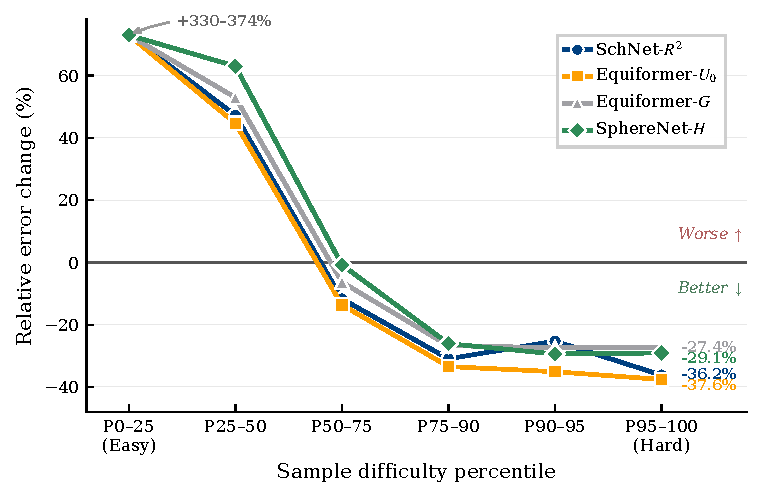
\includegraphics[width=0.55\textwidth]{imgs_edgpp/experiments/difficulty_stratification_lines.pdf}
\caption{Difficulty-stratified relative error change on QM9. All four tasks are plotted on a single panel; the y-axis shows the per-bin relative change in mean absolute error between the tuned-$\kappa$ and default-$\kappa$ configurations. Hard samples (P75--100) show consistent improvement of 25--38\%, while the crossover near P50--75 and the remarkably similar trajectories across architectures confirm that capacity reallocation is a general mechanism of adaptive thresholding. \textit{Note}: P0--25 values are truncated at the y-axis limit; actual relative degradation on easy samples ranges from +330\% to +374\%, but corresponds to negligible absolute error increases.}
\label{fig:difficulty_stratification}
\end{figure}

Figure~\ref{fig:difficulty_stratification} stratifies test samples into six difficulty percentiles and plots the relative per-bin error change for all four representative tasks. The picture is striking: every task traces a nearly identical monotonic descent from degradation on easy samples to improvement on hard samples, crossing zero near P50--75. In relative terms, easy samples (P0--25) suffer a large increase (+330--374\%), whereas hard samples (P95--100) achieve a 27--38\% reduction. Because the absolute errors of easy samples are near-zero under the default-threshold configuration, the large relative increase translates to a negligible absolute penalty; conversely, the moderate relative decrease on hard samples corresponds to a substantial absolute gain.

This difficulty-dependent behavior is the intended mechanism of threshold tuning: by raising $\kappa$ beyond the default, EDG++ applies stricter filtering that suppresses potentially misleading ED signals on samples where the default-threshold model already performs well, reallocating model capacity to under-optimized hard samples. The remarkable consistency of this crossover pattern across three architectures and four quantum properties provides strong evidence that capacity reallocation is a general mechanism of adaptive thresholding.

Robustness metrics further confirm variance reduction: standard deviation reductions of 5.3\% (SchNet-$R^2$), 16.6\% (Equiformer-$U_0$), 17.3\% (Equiformer-$G$), and 11.1\% (SphereNet-$H$). Maximum error reductions are pronounced for Equiformer: 39.1\% ($U_0$) and 37.9\% ($G$). For Equiformer-$U_0$, the maximum error decreases from 1.665 to 1.014, a 39\% reduction that substantially enhances reliability in practical applications.


\section{Property-Type Grouped Analysis}
\label{sec:appendix_property_group}

Table~\ref{tab:property_group} provides a detailed property-type grouped analysis of EDG++ improvements.

\begin{table}[!htb]
  \centering
  \caption{Property-type grouped analysis of EDG++ improvement over the no-distillation baseline on QM9. ``Avg $\Delta$'' denotes the mean relative improvement. ``Win'' denotes the number of properties improved.}
  \label{tab:property_group}
  \scriptsize
  \begin{tabular}{lcccccc}
    \toprule
    \multirow{2}{*}{Group} & \multicolumn{2}{c}{SchNet} & \multicolumn{2}{c}{Equiformer} & \multicolumn{2}{c}{SphereNet} \\
    \cmidrule(lr){2-3} \cmidrule(lr){4-5} \cmidrule(lr){6-7}
    & Avg $\Delta$ & Win & Avg $\Delta$ & Win & Avg $\Delta$ & Win \\
    \midrule
    Electronic & +2.24\% & 5/5 & +3.64\% & 4/5 & +1.96\% & 5/5 \\
    Thermo. & +3.70\% & 5/5 & +16.30\% & 5/5 & +5.52\% & 5/5 \\
    Vibrational & +2.30\% & 1/1 & $-$3.20\% & 0/1 & +4.40\% & 1/1 \\
    Structural & +6.40\% & 1/1 & +11.90\% & 1/1 & +1.90\% & 1/1 \\
    \midrule
    Overall & +3.20\% & 12/12 & +9.03\% & 10/12 & +3.64\% & 12/12 \\
    \bottomrule
  \end{tabular}
\end{table}


\section{Distillation Weight Sensitivity}
\label{sec:appendix_lambda}

Table~\ref{tab:lambda_sensitivity} reports the per-task $\lambda$ sensitivity under the default-threshold configuration.

\begin{table}[!htb]
  \scriptsize
  \centering
  \caption{$\lambda$ sensitivity (relative performance difference between best and worst $\lambda \in \{0.01, 0.5, 1.0\}$) under the default-threshold configuration ($\kappa_{batch}\!=\!\kappa_{all}\!=\!0$, $\beta\!=\!0$).}
  \label{tab:lambda_sensitivity}
    \begin{tabular}{lccc}
    \toprule
    \textbf{Task} & \textbf{SchNet} & \textbf{Equiformer} & \textbf{SphereNet} \\
    \midrule
    $\alpha$   & 1.19\% & 1.21\% & 3.52\% \\
    $C_v$      & 1.09\% & 1.34\% & 1.89\% \\
    $G$        & 2.37\% & 12.85\% & 4.59\% \\
    $\Delta\varepsilon$ & 0.71\% & 1.56\% & 1.74\% \\
    $H$        & 0.33\% & 5.62\% & 6.88\% \\
    $\varepsilon_{\text{HOMO}}$ & 1.79\% & 1.75\% & 0.92\% \\
    $\varepsilon_{\text{LUMO}}$ & 1.39\% & 1.62\% & 2.35\% \\
    $\mu$      & 1.20\% & 3.10\% & 1.94\% \\
    $R^2$      & 2.21\% & 15.26\% & 5.84\% \\
    $U_0$      & 1.94\% & 34.87\% & 7.34\% \\
    $U$        & 1.26\% & 11.06\% & 4.35\% \\
    ZPVE       & 2.21\% & 3.00\% & 0.96\% \\
    \midrule
    \textbf{Average} & \textbf{1.47\%} & \textbf{7.77\%} & \textbf{3.53\%} \\
    \bottomrule
    \end{tabular}
\end{table}


\section{Hyperparameter Configurations for EDG and EDG++}
\label{app:hyper}

We report the default configuration used for the main results in Tables~\ref{tab:rmd17_energy} and~\ref{tab:rmd17_force}, and the full search space in Appendix~\ref{sec:appendix_hyperparam}. On QM9, all three architectures share the same hyperparameter search. On rMD17, all experiments use global thresholding only ($\beta\!=\!0$), because rMD17 trains one model per molecule and every mini-batch is drawn from the conformation distribution of a single molecule; batch-local reliability statistics therefore converge to the global statistics in expectation, and per-batch variation becomes informative only in the multi-molecule QM9 setting (cf.\ Table~\ref{tab:ablation_beta}). An empirical validation of this choice on three representative rMD17 molecules is provided in Appendix~\ref{app:beta_rmd17}. SchNet and ViSNet on rMD17 use the out-of-the-box configuration ($\kappa_{all}\!=\!0$) to probe cross-architecture generality, whereas SphereNet additionally tunes $\kappa_{all}$ per molecule over $\{-1.5, -1, -0.5, 0, 0.5, 1.0, 1.5\}$ to characterize the upper bound of the approach. Per-molecule $\kappa_{all}$ tuning is restricted to SphereNet because the 50-sample rMD17 validation set limits the reliability of such tuning for additional architectures.


\section{Empirical Validation of $\beta\!=\!0$ on rMD17}
\label{app:beta_rmd17}

To validate our default choice of $\beta\!=\!0$ (global-only thresholding) for rMD17, we run a $\beta$ ablation on three representative molecules---Aspirin (large, complex), Salicylic acid (mid-size with hydroxyl groups), and Toluene (small, aromatic)---using SphereNet with $\kappa_{all}\!=\!0$ and $\lambda\!=\!0.001$. Each molecule is trained for 1{,}000 epochs at three values of $\beta\in\{0, 0.5, 1.0\}$. Table~\ref{tab:rmd17_beta_ablation} reports the test-set MAE.

\begin{table}[!htb]
  \scriptsize
  \centering
  \caption{rMD17 $\beta$ ablation on SphereNet ($\kappa_{all}\!=\!0$, $\lambda\!=\!0.001$, 1{,}000 epochs). On the average across three molecules, $\beta\!=\!0$ minimizes Energy MAE while Force MAE is essentially insensitive to $\beta$. On per-molecule basis, $\beta\!=\!0$ is best on Energy for 2/3 molecules with the largest gaps appearing on the more complex molecules (Aspirin and Salicylic). Bold indicates the best result per row.}
  \label{tab:rmd17_beta_ablation}
    \begin{tabular}{lccc}
    \toprule
    \textbf{Molecule} & $\beta\!=\!0$ & $\beta\!=\!0.5$ & $\beta\!=\!1.0$ \\
    \midrule
    \multicolumn{4}{l}{\textit{Energy MAE ($\frac{kcal}{mol}$)}} \\
    Aspirin       & \textbf{0.12406} & 0.18744 & 0.22103 \\
    Salicylic     & \textbf{0.06603} & 0.06894 & 0.09613 \\
    Toluene       & 0.02366 & 0.02252 & \textbf{0.02161} \\
    \emph{Average} & \textbf{0.07125} & 0.09297 & 0.11292 \\
    \midrule
    \multicolumn{4}{l}{\textit{Force MAE ($\frac{kcal}{mol\cdot \text{\r{A}}}$)}} \\
    Aspirin       & \textbf{0.38060} & 0.38130 & 0.38529 \\
    Salicylic     & 0.29756 & \textbf{0.29563} & 0.30040 \\
    Toluene       & 0.10518 & \textbf{0.10428} & 0.10462 \\
    \emph{Average} & 0.26111 & \textbf{0.26040} & 0.26344 \\
    \bottomrule
    \end{tabular}
\end{table}

The aggregate picture supports $\beta\!=\!0$ as the default for rMD17. On Energy MAE, $\beta\!=\!0$ achieves the lowest average error (0.07125 vs.\ 0.09297 for $\beta\!=\!0.5$ and 0.11292 for $\beta\!=\!1$); the gap is largest on the more complex molecules (Aspirin: 51\% lower than $\beta\!=\!0.5$; Salicylic: 4\% lower) and reverses only on Toluene with a small margin (9\% vs.\ $\beta\!=\!1$). On Force MAE, all three $\beta$ values perform within 1\% of each other (the average MAE differs by less than 0.003), reflecting that force prediction is dominated by local atomic interactions rather than the global energy distribution captured by ED. This empirical pattern matches the theoretical motivation in Appendix~\ref{app:hyper}: under per-molecule training, batch-local reliability statistics are noisy estimates of the same global distribution, and the small batch size in rMD17 (4 to 128 conformations of a single molecule) further amplifies noise; pure global thresholding ($\beta\!=\!0$) avoids this noise without losing distributional information.


\section{Progressive Component Ablation (SphereNet, rMD17)}
\label{app:progressive}

To isolate the contribution of the reliability estimator from that of the distillation weight and threshold tuning, we report a progressive-ablation study on SphereNet, the only rMD17 architecture for which the full configuration chain---EDG with tuned $\lambda$, EDG with fixed $\lambda\!=\!0.001$, EDG++ at $\kappa_{all}\!=\!0$, and EDG++ with tuned $\kappa_{all}$---is available. Table~\ref{tab:rmd17_progressive} reports MAE for each configuration.

\begin{table*}[!htb]
  \scriptsize
  \centering
  \caption{Progressive component ablation on SphereNet (rMD17). EDG with tuned $\lambda$ is the conference-version baseline; ``EDG ($\lambda\!=\!0.001$)'' is a controlled baseline sharing the $\lambda$ used by EDG++ but without the reliability estimator; ``EDG++ ($\kappa\!=\!0$)'' denotes the default-threshold EDG++ configuration; ``EDG++'' is the best $\kappa_{all}$ per molecule. Bold indicates the best result per column.}
  \label{tab:rmd17_progressive}
  \setlength{\tabcolsep}{4pt}
    \begin{tabular}{lcccccccccc}
    \toprule
    \textbf{Method} & Aspirin & Azobenz. & Benzene & Ethanol & Malona. & Naphth. & Paracet. & Salicylic & Toluene & Uracil \\
    \midrule
    \multicolumn{11}{l}{\textit{Energy MAE ($\frac{kcal}{mol}$)}} \\
    EDG (tuned $\lambda$) & 0.13622 & \textbf{0.06788} & 0.00413 & \textbf{0.03575} & \textbf{0.05659} & 0.02753 & 0.09934 & 0.09569 & 0.02413 & \textbf{0.03683} \\
    EDG ($\lambda\!=\!0.001$) & 0.18166 & 0.06603 & 0.00377 & 0.04695 & 0.05806 & 0.05216 & 0.10866 & 0.09713 & 0.03175 & 0.05925 \\
    EDG++ ($\kappa\!=\!0$) & 0.12584 & 0.07125 & \textbf{0.00341} & 0.04081 & 0.06767 & 0.02373 & 0.09734 & \textbf{0.06563} & 0.02367 & 0.05570 \\
    EDG++ & \textbf{0.12391} & 0.07125 & \textbf{0.00341} & \textbf{0.03575} & 0.06611 & \textbf{0.02256} & \textbf{0.09628} & \textbf{0.06563} & \textbf{0.02220} & 0.04841 \\
    \midrule
    \multicolumn{11}{l}{\textit{Force MAE ($\frac{kcal}{mol\cdot \text{\r{A}}}$)}} \\
    EDG (tuned $\lambda$) & 0.38598 & \textbf{0.21665} & 0.02101 & 0.18741 & \textbf{0.28456} & 0.11102 & 0.32023 & \textbf{0.28299} & 0.10804 & \textbf{0.17179} \\
    EDG ($\lambda\!=\!0.001$) & 0.38870 & 0.21670 & 0.02160 & \textbf{0.18594} & 0.29120 & 0.11220 & \textbf{0.31742} & 0.28919 & 0.10706 & 0.26561 \\
    EDG++ ($\kappa\!=\!0$) & 0.37960 & 0.22238 & 0.02078 & 0.18871 & 0.31599 & 0.09711 & 0.32309 & 0.29871 & \textbf{0.10341} & 0.23117 \\
    EDG++ & \textbf{0.37929} & 0.21708 & \textbf{0.02012} & 0.18698 & 0.31599 & \textbf{0.09541} & 0.31846 & 0.29452 & \textbf{0.10341} & 0.22544 \\
    \bottomrule
    \end{tabular}
\end{table*}

Comparing EDG ($\lambda\!=\!0.001$) to EDG++ ($\kappa\!=\!0$), which differ only in whether the reliability estimator is active, the estimator improves energy on 8/10 molecules, with naphthalene ($\downarrow$54.5\%), salicylic acid ($\downarrow$32.4\%), and aspirin ($\downarrow$30.7\%) showing the largest gains. Naive distillation at $\lambda\!=\!0.001$ without the estimator degrades energy below baseline on 4/10 molecules (e.g., naphthalene: $\uparrow$36.4\%); the estimator recovers 3 of these 4 cases to below-baseline error, indicating that reliability-aware filtering is essential for safe distillation at this weight. Threshold tuning (EDG++ $\kappa\!=\!0 \to$ EDG++ with tuned $\kappa$) provides further incremental gains.


\section{Boundary Case Analysis: Malonaldehyde}
\label{app:boundary}

Malonaldehyde is the only molecule where the reliability estimator consistently degrades performance on rMD17. Naive distillation at $\lambda\!=\!0.001$ improves energy (0.05806 vs.\ baseline 0.06005, $\downarrow$3.3\%), indicating that the ED-based distillation signal is beneficial for this molecule. Activating the estimator (EDG++ $\kappa\!=\!0$: 0.06767) reverses this gain, suggesting that the estimator incorrectly filters beneficial distillation signal, likely because the rapid intramolecular proton-transfer dynamics of malonaldehyde produce ED patterns that the estimator misclassifies as unreliable. EDG with per-task-best $\lambda$ achieves the best result (0.05659), and threshold tuning partially mitigates the degradation (EDG++ best $\kappa$: 0.06611 versus 0.06767 at $\kappa\!=\!0$), pointing to molecule-adaptive thresholding as a future direction. A per-sample error visualization for malonaldehyde together with two representative success cases (naphthalene, uracil) is given in Appendix~\ref{sec:appendix_rmd17_vis}.


\section{rMD17 Prediction Error Visualization}
\label{sec:appendix_rmd17_vis}

\begin{figure*}[!htb]
\centering
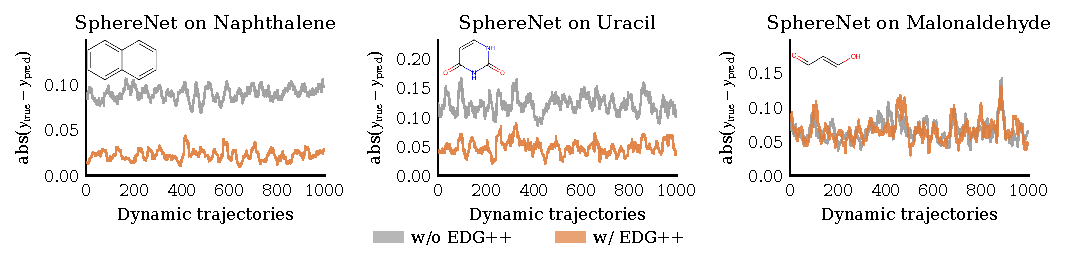
\includegraphics[width=\textwidth]{imgs_edgpp/experiments/rMD17_baseline_vs_edgpp.pdf}
\caption{Per-sample energy prediction errors on rMD17 (SphereNet), comparing the no-distillation baseline with EDG++ ($\kappa_{all}\!=\!1.5$ for naphthalene and uracil; $\kappa_{all}\!=\!1.0$ for malonaldehyde). We include three representative cases: two successes---naphthalene ($\Delta\!=\!+74.9\%$) and uracil ($\Delta\!=\!+60.4\%$)---and the identified boundary case, malonaldehyde ($\Delta\!=\!-0.2\%$), discussed in Appendix~\ref{app:boundary}, where the reliability estimator fails to filter beneficial distillation signal due to the molecule's rapid intramolecular proton-transfer dynamics. \textit{Note}: $\Delta$ values are computed from per-sample predictions of independently trained baseline and EDG++ models, not from the conference-version baselines in Tables~\ref{tab:rmd17_energy}--\ref{tab:rmd17_force}.}
\label{fig:rMD17_vis}
\end{figure*}


\section{Hyperparameter Interaction Analysis}
\label{sec:appendix_heatmap}

\begin{figure*}[!htb]
\centering

\includegraphics[width=\textwidth]{imgs_edgpp/experiments/heatmap_hyperparam.pdf}
\caption{Relative improvement (\%) over the no-distillation baseline as a function of $\kappa_{batch}$ and $\kappa_{all}$ with $\beta=0.5$ on QM9. For each ($\kappa_{batch}$, $\kappa_{all}$) pair, we report the best result across all $\lambda$ values. Blue indicates improvement; red indicates degradation; white corresponds to no change. Bold values denote $|\Delta|>5\%$. \textit{Note}: color scales are independently normalized per panel to maximize contrast within each task-model combination.}
\label{fig:heatmap_hyperparam}
\end{figure*}

Figure~\ref{fig:heatmap_hyperparam} visualizes the relative improvement over the baseline as a function of $\kappa_{batch}$ and $\kappa_{all}$ under the hybrid strategy ($\beta=0.5$) for four representative tasks. Two observations emerge. First, the improvement landscape is generally smooth, with most cells showing positive gains, indicating that EDG++ is robust to the specific choice of $\kappa$ values. Second, the optimal region varies by task and model: for SchNet, the improvements are uniformly distributed (all cells within 1\% of each other), while for SphereNet, thermodynamic properties like $G$ show more pronounced sensitivity to $\kappa_{all}$, with stricter filtering ($\kappa_{all}=1.5$) yielding larger gains.

\textbf{Threshold sensitivity on rMD17.} We further analyze how $\kappa_{all}$ affects energy prediction on rMD17 (SphereNet, $\lambda\!=\!0.001$). The sensitivity patterns are highly molecule-dependent: aspirin and toluene favor negative $\kappa_{all}$ (more inclusive filtering), while naphthalene and uracil favor positive $\kappa_{all}$ (stricter filtering). Malonaldehyde is the most extreme case, with energy improvement fluctuating between $-260\%$ and $+10\%$ across $\kappa_{all} \in [-1.5, 1.5]$, consistent with its challenging proton transfer dynamics. Force predictions are relatively insensitive to $\kappa_{all}$ across all molecules, suggesting that the ED teacher primarily provides global energy-level information rather than local force-level gradients.


\section{ImageED Reconstruction Visualization}
\label{sec:appendix_imageed_vis}

\begin{figure}[!htb]
\centering
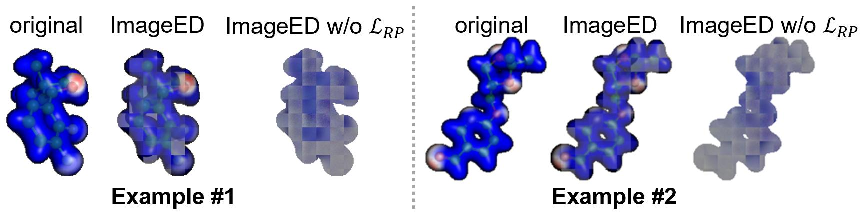
\includegraphics[width=\columnwidth]{imgs_edgpp/experiments/ImageED_output.pdf}
\caption{Visualization of ImageED reconstruction. ImageED generates high-quality ED images compared to the originals. Removing the masked reconstruction task ($\mathcal{L}_{MR}$) limits the understanding of local pixel-level features.}
\label{fig:vis_ImageED}
\end{figure}

Figure~\ref{fig:vis_ImageED} shows the reconstruction quality of ImageED. ImageED can faithfully reconstruct ED images compared to the originals, indicating that it effectively learns ED-related knowledge from the multi-view RGB-D images. Removing the masked reconstruction task (ImageED w/o $\mathcal{L}_{MR}$) degrades the reconstruction of local pixel-level details, confirming the importance of both pretext tasks.


\section{ED Image Representation Comparison}
\label{sec:appendix_ed_repr}

\begin{table}[!htb]
  \scriptsize
  \centering
  \caption{RMSE performance of different ED representations on 6 energy prediction tasks. Point cloud, voxel, and image use PointNet, ResNet3D, and ResNet18, respectively. E1--E6 represent DF-RKS Final Energy, Nuclear Repulsion Energy, One-Electron Energy, Two-Electron Energy, DFT Exchange-Correlation Energy, and Total Energy.}
  \label{tab:results_ED_images}
    \begin{tabular}{ccccccc}
    \toprule
    Repr. & E1 & E2 & E3 & E4 & E5 & E6 \\
    \midrule
    Point & 275.1 & 168.6 & 557.7 & 244.8 & 14.5 & 288.9 \\
    Voxel & 121.1 & 313.9 & 947.8 & 271.2 & 7.9 & 202.0 \\
    Image & \textbf{111.6} & \textbf{47.9} & \textbf{349.8} & \textbf{85.6} & \textbf{4.4} & \textbf{124.5} \\
    \midrule
    $\Delta$ & $\uparrow$7.8\% & $\uparrow$71.6\% & $\uparrow$37.3\% & $\uparrow$65.0\% & $\uparrow$44.5\% & $\uparrow$38.4\% \\
    \bottomrule
    \end{tabular}
\end{table}


\section{Computational Cost Analysis}
\label{sec:appendix_cost}

EDG++ introduces no additional parameters or forward passes beyond EDG; the only overhead is a scalar reliability score lookup per sample, resulting in $<$5\% per-epoch overhead compared to the no-distillation baseline. All experiments were conducted on 8$\times$ NVIDIA H200 GPUs. On QM9, a single distillation run takes $\sim$18h (SchNet, 1000 epochs), $\sim$35h (SphereNet, 1000 epochs), or $\sim$40h (Equiformer, 300 epochs). The dominant cost is the grid search: each model requires 45 configurations (3 $\lambda$ values $\times$ 15 $(\kappa, \beta)$ combinations) per task, totaling $\sim$9.6k, $\sim$19.0k, and $\sim$21.3k GPU-hours for SchNet, SphereNet, and Equiformer, respectively. On rMD17, SphereNet requires 7 $\kappa_{all}$ values per molecule ($\sim$46h per run), totaling $\sim$3.1k GPU-hours. In practice, the search can be substantially reduced by first identifying a good $\lambda$ on a representative task and then only searching over $(\kappa, \beta)$, which would reduce the search space by 3$\times$.


\section{Contribution Decomposition and Baseline Discussion}
\label{sec:appendix_contribution}

Our experimental design provides a natural two-level decomposition: Baseline $\to$ EDG isolates the contribution of ED as privileged information, and EDG $\to$ EDG++ isolates the contribution of reliability-aware selective distillation.

\textbf{Why standard KD baselines are not included.} We acknowledge that comparisons with adapted standard KD baselines (\eg, FitNets~\cite{romero2015fitnets}, AT~\cite{zagoruyko2017paying}) would strengthen the paper. In principle, one could implement a ``structural-image teacher $\to$ geometry student'' feature matching control without ED pre-training, which would help disentangle whether the gains come from (1)~the ED signal itself, (2)~the auxiliary teacher architecture, or (3)~the cross-modal training paradigm. We did not include such controls due to computational budget constraints: the full EDG++ grid search already required $\sim$50k GPU-hours.

However, several lines of indirect evidence support that the gains primarily originate from the ED signal rather than the teacher architecture \emph{per se}: (i)~the improvement hierarchy across property types (thermodynamic $>$ electronic $>$ vibrational) is physically consistent with the Hohenberg-Kohn theorem---a generic teacher architecture would not produce this pattern; (ii)~the improvements are consistent across four fundamentally different student architectures (SchNet, Equiformer, SphereNet, ViSNet), suggesting the transferred knowledge is architecture-agnostic; (iii)~the reliability estimator, trained to predict \emph{ED reconstruction error}, is effective at identifying samples where distillation helps---this would not work if the gains were unrelated to ED quality. We encourage future work to include a non-ED teacher control to formally validate this decomposition.


\section{Dataset Descriptions}
\label{sec:appendix_datasets}

\subsection{QM9 Dataset}

QM9~\cite{ramakrishnan2014quantum} is a widely used benchmark for quantum chemistry, containing 133,885 small organic molecules with up to 9 heavy atoms (C, N, O, F). Each molecule is associated with 12 quantum mechanical properties computed using density functional theory (DFT) at the B3LYP/6-31G(2df,p) level. Table~\ref{tab:qm9_properties} provides detailed descriptions of these properties.

\begin{table}[!htb]
  \centering
  \caption{Descriptions of 12 quantum mechanical properties in QM9.}
  \label{tab:qm9_properties}
  \scriptsize
    \begin{tabular}{clcc}
    \toprule
    \textbf{Property} & \textbf{Description} & \textbf{Unit} & \textbf{Type} \\
    \midrule
    $\alpha$ & Isotropic polarizability & $a_0^3$ & Electronic \\
    $\Delta\varepsilon$ & HOMO-LUMO gap & meV & Electronic \\
    $\varepsilon_{HOMO}$ & Highest occupied molecular orbital energy & meV & Electronic \\
    $\varepsilon_{LUMO}$ & Lowest unoccupied molecular orbital energy & meV & Electronic \\
    $\mu$ & Dipole moment & D & Electronic \\
    $C_v$ & Heat capacity at 298.15K & $\frac{cal}{mol \cdot K}$ & Thermodynamic \\
    $G$ & Free energy at 298.15K & meV & Thermodynamic \\
    $H$ & Enthalpy at 298.15K & meV & Thermodynamic \\
    $R^2$ & Electronic spatial extent & $a_0^2$ & Structural \\
    $U$ & Internal energy at 298.15K & meV & Thermodynamic \\
    $U_0$ & Internal energy at 0K & meV & Thermodynamic \\
    ZPVE & Zero point vibrational energy & meV & Vibrational \\
    \bottomrule
    \end{tabular}
\end{table}

\subsection{rMD17 Dataset}

The revised MD17 (rMD17)~\cite{christensen2020role} dataset contains molecular dynamics trajectories for 10 small organic molecules. Each trajectory consists of molecular conformations with corresponding energies and atomic forces computed at the PBE+vdW-TS level of theory. Table~\ref{tab:rmd17_molecules} provides detailed descriptions of these molecules.

\begin{table}[!htb]
  \centering
  \caption{Descriptions of 10 molecules in rMD17.}
  \label{tab:rmd17_molecules}
  \scriptsize
    \begin{tabular}{clccc}
    \toprule
    \textbf{No.} & \textbf{Molecule} & \textbf{Formula} & \textbf{\#Atoms} & \textbf{\#Conformations} \\
    \midrule
    1 & Aspirin & C$_9$H$_8$O$_4$ & 21 & 211,762 \\
    2 & Azobenzene & C$_{12}$H$_{10}$N$_2$ & 24 & 99,999 \\
    3 & Benzene & C$_6$H$_6$ & 12 & 627,983 \\
    4 & Ethanol & C$_2$H$_6$O & 9 & 555,092 \\
    5 & Malonaldehyde & C$_3$H$_4$O$_2$ & 9 & 993,237 \\
    6 & Naphthalene & C$_{10}$H$_8$ & 18 & 326,250 \\
    7 & Paracetamol & C$_8$H$_9$NO$_2$ & 20 & 106,490 \\
    8 & Salicylic acid & C$_7$H$_6$O$_3$ & 16 & 320,231 \\
    9 & Toluene & C$_7$H$_8$ & 15 & 442,790 \\
    10 & Uracil & C$_4$H$_4$N$_2$O$_2$ & 12 & 133,770 \\
    \bottomrule
    \end{tabular}
\end{table}


\section{Paired Bootstrap Confidence Intervals}
\label{sec:appendix_bootstrap}

To quantify the estimation uncertainty of our single-seed results, we compute paired bootstrap 95\% confidence intervals based on per-sample test predictions (10,831 samples for QM9). For each task-model pair, we resample the test set 10,000 times with replacement and compute the MAE on each resample. Table~\ref{tab:bootstrap_ci} reports the bootstrap CI for representative tasks.

\begin{table}[!htb]
  \centering
  \caption{Bootstrap 95\% CIs for EDG++ (per-task-best) and paired bootstrap test of EDG++ vs.\ EDG on representative QM9 tasks. $\Delta$: paired difference in MAE (EDG $-$ EDG++; positive means EDG++ is better).}
  \label{tab:bootstrap_ci}
  \scriptsize
  \begin{tabular}{llccc}
    \toprule
    \textbf{Model} & \textbf{Task} & \textbf{EDG++ MAE [95\% CI]} & \textbf{$\Delta$ [95\% CI]} & \textbf{$p$} \\
    \midrule
    SchNet & $R^2$ & 0.126 [0.121, 0.132] & +0.003 [+0.000, +0.006] & 0.020 \\
    Equif. & $U_0$ & 0.017 [0.016, 0.018] & +0.001 [+0.001, +0.002] & $<$0.001 \\
    Equif. & $\mu$ & 0.021 [0.020, 0.022] & 0.000 & n.s. \\
    Sphere. & $H$ & 0.006 [0.006, 0.007] & +0.000 [$-$0.000, +0.000] & 0.472 \\
    Sphere. & ZPVE & 0.001 [0.001, 0.001] & +0.000 [+0.000, +0.000] & 0.003 \\
    \bottomrule
  \end{tabular}
\end{table}

The mean relative CI width across all 36 task-model pairs is 7.0\% (median 6.1\%, max 12.5\%), indicating that the single-seed point estimates are reasonably stable. The paired bootstrap tests confirm that several key improvements (Equiformer-$U_0$, SphereNet-ZPVE) are statistically robust even within a single seed ($p < 0.01$), while others (SphereNet-$H$) require multi-seed evaluation for definitive conclusions.


\section{Hyperparameter Search Space}
\label{sec:appendix_hyperparam}

We conduct grid search over the following hyperparameters for EDG++:

\begin{itemize}
    \item \textbf{Distillation weight} $\lambda \in \{0.01, 0.5, 1.0\}$ for QM9; $\lambda = 0.001$ for rMD17
    \item \textbf{Local threshold coefficient} $\kappa_{batch} \in \{-1.5, 0, 1.5\}$
    \item \textbf{Global threshold coefficient} $\kappa_{all} \in \{-1.5, 0, 1.5\}$ for QM9; $\{-1.5, -1, -0.5, 0, 0.5, 1.0, 1.5\}$ for rMD17
    \item \textbf{Mixing coefficient} $\beta \in \{0, 0.5, 1.0\}$ for QM9; $\beta = 0$ for rMD17
\end{itemize}

For each task, we select the hyperparameter configuration that achieves the best validation performance.


\section{Implementation Details}
\label{sec:appendix_implementation}

\subsection{ImageED Pre-training}

The encoder and decoder of ImageED are built based on ViT-Base/16~\cite{dosovitskiy2020image}. The encoder has an embedding dimension of 768 with 12 Transformer layers, and the decoder has an embedding dimension of 512 with 8 Transformer layers. We use a learning rate of 1.5e-4, a batch size of 64, a mask ratio of 0.25, $\lambda_{VR}=1$ and $\lambda_{MR}=1$ for 20 epochs on 8 GeForce RTX 4090 GPUs. The input ED images have shape $6 \times 4 \times 224 \times 224$ (6 views, 4 channels including RGB-D).

\subsection{ED-aware Teacher Pre-training}

We divide 2\% of the 2 million molecules as validation set and the rest as training set. The ED-aware teacher uses ResNet18~\cite{he2016deep} with view-wise average pooling. The ED predictor is a 2-layer MLP with Softplus activation. We use a learning rate of 5e-3 and a batch size of 128 to train for approximately 280k steps.

\subsection{Reliability Estimator Training}

The reliability estimator is a lightweight MLP with architecture: Linear(512, 256) $\rightarrow$ Softplus $\rightarrow$ Linear(256, 1), with approximately 131K parameters. It is jointly trained with the ED-aware teacher and ED predictor in Stage II, sharing the same SGD optimizer (momentum 0.9, learning rate 0.003, weight decay 1e-4, batch size 128, 25 epochs). Note that the evaluator's input features are detached from the teacher's computation graph to prevent gradient interference. The training objective is to predict the L2 reconstruction error between predicted and ground-truth ED features.

\subsection{Downstream Task Training}

For QM9, we use the dataset split from Geom3D~\cite{liu2024symmetry}: 110K for training, 10K for validation, and 11K for testing. For rMD17, we use 950 for training, 50 for validation, and 1000 for testing. The mapper $f_M$ and task predictor $f_T$ each consist of a single linear layer. We select the best checkpoint based on validation MAE for QM9 and validation force MAE for rMD17.
